\documentclass[12pt,letterpaper]{article}

%% --- Packages -----------------------------------------------------------------
\usepackage[margin=1in]{geometry}
\usepackage{amsmath,amssymb,amsthm}
\usepackage{mathtools}
\usepackage[T1]{fontenc}
\usepackage[utf8]{inputenc}
\usepackage{hyperref}
\usepackage{listings}
\usepackage{xcolor}
\usepackage{booktabs}
\usepackage{array}
\usepackage{longtable}
\usepackage{enumitem}
\usepackage{titlesec}
\usepackage{fancyhdr}
\usepackage{graphicx}
\usepackage{tikz}
\usetikzlibrary{shapes.geometric,arrows,positioning,fit,backgrounds}
\usepackage{tcolorbox}
\usepackage{mdframed}
\usepackage{cleveref}
\usepackage{setspace}
%\usepackage[protrusion=true]{microtype}
\usepackage{abstract}

%% --- Colours ------------------------------------------------------------------
\definecolor{primeblue}{RGB}{30,80,160}
\definecolor{codegray}{RGB}{245,245,245}
\definecolor{codered}{RGB}{180,30,30}
\definecolor{codegreen}{RGB}{20,120,60}
\definecolor{codepurple}{RGB}{100,30,160}
\definecolor{alertorange}{RGB}{220,100,0}

%% --- Hyperref -----------------------------------------------------------------
\hypersetup{
  colorlinks=true,
  linkcolor=primeblue,
  citecolor=primeblue,
  urlcolor=primeblue,
  pdftitle={PIRTM Policy Packs: Mathematically Grounded Compliance Framework},
  pdfauthor={Ryan Van Gelder --- Multiplicity Foundation},
  pdfsubject={Defensive Publication / Prior Art},
}

%% --- Listings style -----------------------------------------------------------
\lstdefinestyle{jsonStyle}{
  backgroundcolor=\color{codegray},
  basicstyle=\ttfamily\small,
  keywordstyle=\color{primeblue}\bfseries,
  stringstyle=\color{codered},
  commentstyle=\color{codegreen}\itshape,
  numberstyle=\tiny\color{gray},
  numbers=left,
  stepnumber=1,
  breaklines=true,
  frame=single,
  rulecolor=\color{gray!40},
  captionpos=b,
  morekeywords={true,false,null},
  literate=
    *{0}{{{\color{codepurple}0}}}1
     {1}{{{\color{codepurple}1}}}1
     {2}{{{\color{codepurple}2}}}1
     {3}{{{\color{codepurple}3}}}1
}

\lstdefinestyle{pythonStyle}{
  backgroundcolor=\color{codegray},
  basicstyle=\ttfamily\small,
  keywordstyle=\color{primeblue}\bfseries,
  stringstyle=\color{codered},
  commentstyle=\color{codegreen}\itshape,
  numberstyle=\tiny\color{gray},
  numbers=left,
  stepnumber=1,
  breaklines=true,
  frame=single,
  rulecolor=\color{gray!40},
  captionpos=b,
  language=Python,
}

\lstdefinestyle{bnfStyle}{
  backgroundcolor=\color{codegray},
  basicstyle=\ttfamily\small,
  keywordstyle=\color{codepurple}\bfseries,
  commentstyle=\color{codegreen}\itshape,
  numbers=left,
  stepnumber=1,
  breaklines=true,
  frame=single,
  rulecolor=\color{gray!40},
  captionpos=b,
}

%% --- Theorem environments -----------------------------------------------------
\theoremstyle{definition}
\newtheorem{definition}{Definition}[section]
\newtheorem{axiom}{Axiom}[section]
\theoremstyle{plain}
\newtheorem{theorem}{Theorem}[section]
\newtheorem{lemma}[theorem]{Lemma}
\newtheorem{corollary}[theorem]{Corollary}
\newtheorem{proposition}[theorem]{Proposition}
\theoremstyle{remark}
\newtheorem{remark}{Remark}[section]
\newtheorem{example}{Example}[section]

%% --- Custom boxes -------------------------------------------------------------
\tcbuselibrary{breakable,skins}
\newtcolorbox{policybox}[1]{
  colback=primeblue!5,
  colframe=primeblue,
  fonttitle=\bfseries,
  title=#1,
  breakable,
}
\newtcolorbox{warnbox}[1]{
  colback=alertorange!10,
  colframe=alertorange,
  fonttitle=\bfseries,
  title=#1,
}

%% --- Page style ---------------------------------------------------------------
\pagestyle{fancy}
\fancyhf{}
\lhead{\small PIRTM Policy Packs --- Defensive Publication}
\rhead{\small Multiplicity Foundation \textcopyright\ 2026}
\cfoot{\thepage}
\setlength{\headheight}{14pt}

%% --- Title --------------------------------------------------------------------
\title{
  \vspace{-0.5in}
  {\LARGE \textbf{PIRTM Policy Packs:}} \\[6pt]
  {\large A Mathematically Grounded Compliance Framework} \\[4pt]
  {\large via Prime-Indexed Recursive Tensor Mathematics,} \\[2pt]
  {\large Phase Mirror Governance, and Formal Policy Semantics} \\[12pt]
  \rule{\textwidth}{0.5pt} \\[6pt]
  {\normalsize \textit{Defensive Publication --- Prior Art Disclosure}} \\[4pt]
  {\normalsize Document ID: \texttt{MF-2026-001-PIRTM-POLICY}} \\[2pt]
  {\normalsize Publication Date: April 25, 2026}
}
\author{
  Phase Mirror Research Initiative \\ \\
  \textit{Citizen Gardens} \\
  \textit{The Foundation of Multiplicity} \\[4pt]
}
\date{April 25, 2026}

%% ===============================================================================
\begin{document}
\maketitle
\thispagestyle{fancy}

\begin{abstract}
\noindent
This document constitutes a \textbf{defensive prior art publication} disclosing the
conceptual framework, mathematical foundations, formal architecture, and
implementation strategy for \emph{PIRTM Policy Packs}: a system for translating
regulatory compliance standards (including FDA 21 CFR, HIPAA, PII, PHI, FHIR HL7,
and ISO 27001) into mathematically precise, machine-checkable, and auditable
formal specifications using the \emph{Prime-Indexed Recursive Tensor Mathematics}
(PIRTM) runtime and the \emph{Phase Mirror} governance protocol.

The central claim of this disclosure is that \textbf{a policy is precisely the
human-language description of a mathematical invariant}; translating it into
mathematics does not alter its intent --- it makes its intent checkable. The
disclosure covers: a three-layer formal policy stack (grammar, predicate schema,
state-transition model); a policy DSL with JSON Schema wrapper optimised for
auditability; the binding of compliance controls to prime-indexed recursive
identities; and a multi-agent pipeline for automated policy formalisation and
evidence generation. By publishing this disclosure, all described concepts are
placed irrevocably in the public domain as prior art, preventing downstream
patent capture of these methods.
\end{abstract}

\tableofcontents
\newpage

%% ===============================================================================
\section{Executive Summary}
\label{sec:exec}

Regulatory compliance in healthcare, life sciences, and data governance is
dominated by natural language documents. These documents are ambiguous, expensive
to audit, and resistant to automated verification. The PIRTM Policy Pack
framework addresses this gap by establishing a \emph{formal translation path}
from regulatory text to machine-checkable mathematical objects.

The architecture proceeds through three strictly separated layers:

\begin{enumerate}[leftmargin=2em]
  \item \textbf{Grammar Layer} --- A domain-specific language (DSL) and
  Backus-Naur Form (BNF) grammar that assigns unambiguous syntactic structure to
  any policy statement. This layer does not carry semantics; it names policy
  elements.

  \item \textbf{Predicate Schema Layer} --- Each grammar token is bound to a
  first-order predicate or a PIRTM-encoded invariant. This layer transforms
  syntactic names into truth-valued mathematical objects that can be checked
  automatically.

  \item \textbf{State-Transition Layer} --- Policy enforcement over time is
  modelled as a labelled transition system. Transitions are admitted only after
  their associated invariants pass. This layer governs dynamic compliance
  behaviour without fusing it with static intent.
\end{enumerate}

The binding mechanism across all three layers is the \emph{Phase Mirror
protocol}: a recursive governance structure in which each layer reflects, checks,
and emits audit evidence before the next layer is activated. Compliance becomes
not a periodic audit event but a continuously verifiable property of the system
state.

The target policy packs disclosed herein cover six regulatory domains:

\begin{center}
\begin{tabular}{lll}
\toprule
\textbf{Pack} & \textbf{Domain} & \textbf{Primary Standard} \\
\midrule
\texttt{PP-FDA}   & Pharmaceutical/Device & FDA 21 CFR Parts 11, 820 \\
\texttt{PP-HIPAA} & Healthcare Privacy     & HIPAA Privacy \& Security Rules \\
\texttt{PP-PII}   & Data Identity          & NIST SP 800-188, GDPR Art.\ 4 \\
\texttt{PP-PHI}   & Protected Health Info  & 45 CFR 164.514, 18 HIPAA Identifiers \\
\texttt{PP-FHIR}  & Interoperability       & HL7 FHIR R4 / 21st Century Cures Act \\
\texttt{PP-ISO}   & Info Security Mgmt     & ISO/IEC 27001:2022 \\
\bottomrule
\end{tabular}
\end{center}

%% ===============================================================================
\section{Motivation and Theoretical Basis}
\label{sec:motivation}

\subsection{Mathematics as Precise Policy}
\label{subsec:mathaspolicy}

The central insight driving this framework is deceptively simple:

\begin{policybox}{Core Thesis}
\textit{Mathematics is what a policy looks like when it is written down
precisely.}

A policy written in natural language is an approximation of an invariant. When
translated into formal mathematics, the invariant becomes checkable. The policy
does not change in intent; it becomes falsifiable.
\end{policybox}

This observation unifies two domains that have historically operated in
isolation: the domain of regulatory compliance (governed by lawyers and auditors)
and the domain of formal verification (governed by mathematicians and engineers).
The PIRTM Policy Pack framework provides the translation layer between them.

\subsection{Multiplicity Theory and Prime Indexing}

Multiplicity Theory, as developed under the Multiplicity Foundation, treats
mathematical objects as \emph{recursively generated patterns of prime-labeled
interactions}. A set is not merely a collection of elements; it is a
\emph{multiplicity space} in which identity, frequency, and relational structure
are preserved across recursive feedback loops through prime-number decomposition.

Formally, a multiplicity space $\mathcal{M}$ over prime set
$\mathcal{P} = \{p_1, p_2, p_3, \ldots\}$ is defined as:

\begin{equation}
\mathcal{M} = \left\{ p_1^{m_1},\, p_2^{m_2},\, \ldots,\, p_n^{m_n} \right\},
\quad m_i \in \mathbb{N}_0
\label{eq:mspace}
\end{equation}

where each $p_i$ encodes the \emph{identity} of a system component and $m_i$
encodes its \emph{multiplicity} (frequency of occurrence or interaction weight).
The key stability property follows from the Fundamental Theorem of Arithmetic:

\begin{theorem}[Prime-Index Stability]
For any two multiplicity spaces $\mathcal{M}_1$ and $\mathcal{M}_2$, the
composition operation
\begin{equation}
\mathcal{M}_1 \otimes \mathcal{M}_2 = \left\{ p_i^{m_i + m'_i} \right\}
\label{eq:compose}
\end{equation}
preserves the unique identity of every component, is associative, and is
invertible over $\mathbb{Q}^+$.
\end{theorem}

\begin{proof}
By the Fundamental Theorem of Arithmetic, the prime factorisation of any
positive integer is unique. Hence the exponent $m_i + m'_i$ uniquely identifies
the combined interaction weight of component $p_i$. Associativity follows from
commutativity of integer addition. Invertibility over $\mathbb{Q}^+$ follows
from allowing negative exponents.
\end{proof}

\subsection{Why Prime Indexing for Compliance}

Compliance policy controls share structural properties with prime-indexed
systems:

\begin{itemize}
  \item \textbf{Atomicity} --- Each control is irreducible; it cannot be
  partially satisfied.
  \item \textbf{Composability} --- Controls from different frameworks combine
  without ambiguity.
  \item \textbf{Auditability} --- The prime-index of each control provides a
  unique, collision-resistant identifier for audit trails.
  \item \textbf{Recursive Stability} --- Repeated application of a control (e.g.,
  periodic re-certification) does not alter the control's identity; only its
  multiplicity exponent changes.
\end{itemize}

%% ===============================================================================
\section{The Three-Layer Formal Policy Stack}
\label{sec:stack}

\subsection{Layer Architecture Overview}

The three layers are strictly ordered and non-fusing. Each layer has a
well-defined input interface, output contract, and failure mode. No layer may
carry the concerns of another in version 1 of any policy pack.

\begin{center}
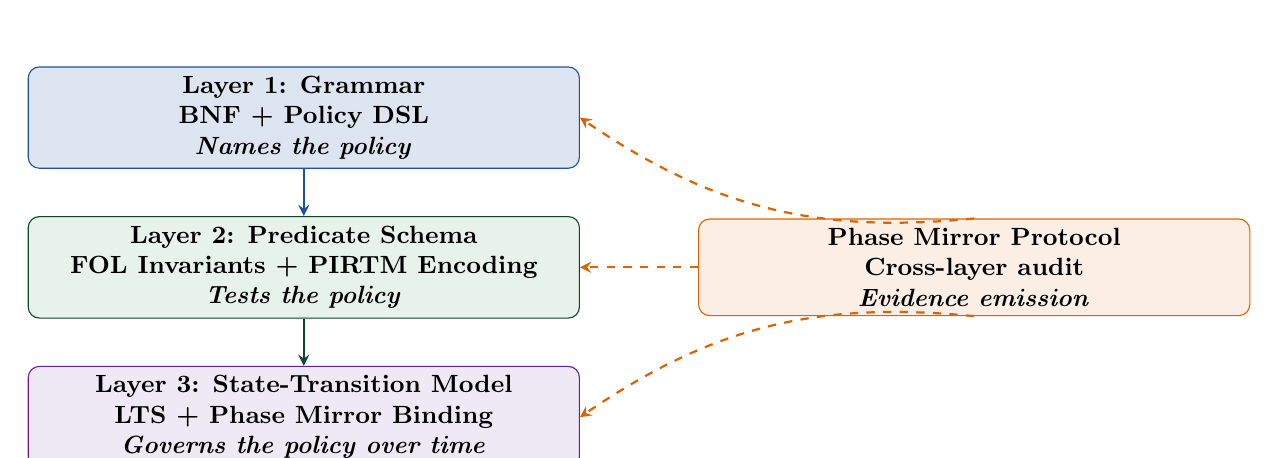
\begin{tikzpicture}[
  box/.style={rectangle, rounded corners=4pt, minimum width=7cm,
    minimum height=1.1cm, draw, align=center, font=\small\bfseries},
  arrow/.style={->,>=stealth,thick}
]
\node[box, fill=primeblue!15, draw=primeblue] (g)
  {\textbf{Layer 1: Grammar} \\ BNF + Policy DSL \\ \textit{Names the policy}};
\node[box, fill=codegreen!10, draw=codegreen!60!black, below=0.6cm of g] (p)
  {\textbf{Layer 2: Predicate Schema} \\ FOL Invariants + PIRTM Encoding \\
   \textit{Tests the policy}};
\node[box, fill=codepurple!10, draw=codepurple, below=0.6cm of p] (s)
  {\textbf{Layer 3: State-Transition Model} \\ LTS + Phase Mirror Binding \\
   \textit{Governs the policy over time}};
\node[box, fill=alertorange!10, draw=alertorange, right=1.5cm of p] (pm)
  {\textbf{Phase Mirror Protocol} \\ Cross-layer audit \\ \textit{Evidence emission}};
\draw[arrow, primeblue] (g) -- (p);
\draw[arrow, codegreen!60!black] (p) -- (s);
\draw[arrow, dashed, alertorange] (pm.west) -- (p.east);
\draw[arrow, dashed, alertorange, bend left=20] (pm.north) to (g.east);
\draw[arrow, dashed, alertorange, bend right=20] (pm.south) to (s.east);
\end{tikzpicture}
\end{center}

\subsection{Layer 1 --- Grammar}

The Grammar Layer establishes the legal syntactic shape of any policy statement
within the PIRTM Policy Pack system. It is specified in two complementary
notations:

\begin{enumerate}
  \item \textbf{BNF} for human-authored syntax definition and documentation.
  \item \textbf{JSON Schema} for machine-validation of policy document
  structure.
\end{enumerate}

\begin{definition}[Policy Statement]
A \emph{policy statement} $\Pi$ is a 5-tuple:
\begin{equation}
\Pi = \langle \mathtt{subject},\; \mathtt{action},\;
              \mathtt{data\_class},\; \mathtt{constraint},\;
              \mathtt{exception} \rangle
\label{eq:policystatement}
\end{equation}
where each component is drawn from a closed vocabulary defined by the relevant
regulatory domain.
\end{definition}

\subsubsection{BNF Grammar for Policy Statements}

\begin{lstlisting}[style=bnfStyle, caption={Core BNF grammar for PIRTM Policy DSL v1}]
<policy>       ::= <header> <body>+
<header>       ::= "policy" <id> ":" <framework> <version>
<id>           ::= <alpha> (<alpha> | <digit> | "-")*
<framework>    ::= "FDA" | "HIPAA" | "PII" | "PHI" | "FHIR" | "ISO"
<version>      ::= "v" <digit>+ "." <digit>+
<body>         ::= <rule>+
<rule>         ::= "rule" <id> ":" <subject> <action> <data-class>
                   <constraint> [<exception>]
<subject>      ::= "subject" ":" <entity>
<entity>       ::= "covered_entity" | "business_associate"
                 | "agent" | "system" | "user"
<action>       ::= "action" ":" <verb>
<verb>         ::= "read" | "write" | "transmit" | "store"
                 | "delete" | "de-identify" | "audit" | "disclose"
<data-class>   ::= "data" ":" <class-id>+
<class-id>     ::= "PHI" | "PII" | "ePHI" | "PQC" | "audit-log"
                 | "device-record" | "FHIR-resource"
<constraint>   ::= "when" ":" <predicate>
<predicate>    ::= <atom> | <predicate> "AND" <predicate>
                 | <predicate> "OR" <predicate>
                 | "NOT" <predicate> | "(" <predicate> ")"
<atom>         ::= <field> <op> <value>
<field>        ::= <alpha> (<alpha> | "_")*
<op>           ::= "==" | "!=" | "<" | ">" | "<=" | ">=" | "in" | "matches"
<value>        ::= <string> | <number> | <list>
<exception>    ::= "except" ":" <predicate>
<alpha>        ::= [a-zA-Z]+
<digit>        ::= [0-9]+
\end{lstlisting}

\subsection{Layer 2 --- Predicate Schema}

Each grammar token is mapped to a first-order predicate. The predicate schema
encodes the \emph{truth conditions} for a policy rule: under what exact
mathematical conditions the rule is satisfied, violated, or indeterminate.

\begin{definition}[Compliance Predicate]
For a rule $r$ over data instance $d$, subject $s$, and context $c$, the
compliance predicate is a function:
\begin{equation}
\Phi_r : D \times S \times C \rightarrow \{0, 1, \bot\}
\label{eq:complpred}
\end{equation}
where $\bot$ denotes an indeterminate state requiring human review.
\end{definition}

\begin{definition}[PIRTM Policy Invariant]
A policy pack $\mathcal{PP}_k$ for regulatory framework $k$ is a set of
prime-indexed invariants:
\begin{equation}
\mathcal{PP}_k = \left\{ \left( p_i^{(k)},\; \Phi_{r_i}^{(k)} \right) \mid
  i = 1, 2, \ldots, N_k \right\}
\label{eq:packdef}
\end{equation}
where $p_i^{(k)}$ is the unique prime index of control $r_i$ within framework
$k$, and $\Phi_{r_i}^{(k)}$ is its compliance predicate.
\end{definition}

The full compliance state of a system $\mathcal{S}$ against pack
$\mathcal{PP}_k$ is:
\begin{equation}
\Gamma(\mathcal{S},\, \mathcal{PP}_k) =
  \bigwedge_{i=1}^{N_k} \Phi_{r_i}^{(k)}(d_i, s_i, c_i)
\label{eq:compliancestate}
\end{equation}

A system is \emph{compliant} with pack $k$ if and only if
$\Gamma(\mathcal{S}, \mathcal{PP}_k) = 1$.

\subsubsection{Example: PHI Predicate Encoding}

The 18 HIPAA identifiers define the boundary of Protected Health Information.
In PIRTM predicate form, this becomes:

\begin{equation}
\Phi_{\text{PHI-001}}(d) =
  \begin{cases}
    1 & \text{if } d \text{ contains no element from } \mathcal{I}_{18} \\
    0 & \text{if } \exists\, x \in d \text{ such that } x \in \mathcal{I}_{18} \\
    \bot & \text{if context linkage is ambiguous}
  \end{cases}
\label{eq:phipred}
\end{equation}

where $\mathcal{I}_{18} = \{ \text{name}, \text{SSN}, \text{DOB}, \ldots \}$ is
the set of 18 HIPAA-defined identifiers.

\subsection{Layer 3 --- State-Transition Model}

Policy enforcement over time is modelled as a Labelled Transition System (LTS).
A state in the LTS represents the current compliance posture of the system; a
transition represents a data event, an agent action, or a certification event.

\begin{definition}[Compliance LTS]
The compliance LTS for pack $\mathcal{PP}_k$ is a 4-tuple:
\begin{equation}
\mathcal{L}_k = (Q_k,\; \Sigma_k,\; \delta_k,\; q_0^{(k)})
\label{eq:lts}
\end{equation}
where:
\begin{itemize}
  \item $Q_k$ is the finite set of compliance states
  $\{\text{COMPLIANT}, \text{PENDING}, \text{VIOLATION}, \text{EXCEPTION}\}$
  \item $\Sigma_k$ is the alphabet of policy-relevant events
  \item $\delta_k : Q_k \times \Sigma_k \rightarrow Q_k$ is the transition
  function, gated by predicate checks
  \item $q_0^{(k)} = \text{PENDING}$ is the initial state before first
  attestation
\end{itemize}
\end{definition}

\begin{axiom}[Transition Gate]
A transition $q \xrightarrow{\sigma} q'$ is admitted in $\mathcal{L}_k$ if and
only if:
\begin{equation}
\Phi_\sigma(d, s, c) = 1 \quad \wedge \quad \text{AuditRecord}(\sigma) \neq
\emptyset
\label{eq:gate}
\end{equation}
That is, the predicate for the triggering event must evaluate to true, and a
non-empty audit record must exist.
\end{axiom}

%% ===============================================================================
\section{Phase Mirror Protocol Binding}
\label{sec:phasemirror}

\subsection{Protocol Description}

The Phase Mirror (PM) protocol is the governance mechanism that binds the three
layers into a single auditable pipeline. It operates as a recursive
\emph{reflection-check-emit} cycle:

\begin{enumerate}
  \item \textbf{Reflect} --- Each layer receives a policy object from the layer
  above and checks structural correctness against its own contract.
  \item \textbf{Check} --- The layer evaluates its associated predicates or
  invariants against the current system state.
  \item \textbf{Emit} --- If the check passes, the layer emits a signed, timestamped
  audit record and passes the policy object to the next layer.
\end{enumerate}

\subsection{Formal PM Binding Equation}

Let $\Lambda = (\Lambda_1, \Lambda_2, \Lambda_3)$ denote the three-layer stack.
The Phase Mirror binding is the composition:

\begin{equation}
\text{PM}(\Pi) = \Lambda_3\!\left(\Lambda_2\!\left(\Lambda_1(\Pi)\right)\right)
\label{eq:pmbind}
\end{equation}

with the constraint that $\Lambda_{i+1}$ is called only if $\Lambda_i$ emits
status $\texttt{PASS}$. If any layer emits $\texttt{FAIL}$, the pipeline halts
and a structured violation record is generated.

\subsection{Recursive Stability Under PM}

\begin{theorem}[PM Recursive Stability]
If each layer predicate $\Phi_i$ is a decidable predicate over finite data, then
the Phase Mirror pipeline $\text{PM}(\Pi)$ terminates for all well-formed inputs
$\Pi$ in finite time.
\end{theorem}

\begin{proof}
(Sketch) Each layer performs a finite evaluation over a bounded data structure.
By induction on the layer index: $\Lambda_1$ terminates because BNF parsing of
finite strings is decidable. $\Lambda_2$ terminates because first-order predicate
evaluation over finite domains is decidable. $\Lambda_3$ terminates because
transition evaluation over a finite-state LTS is decidable. The composition
of three terminating functions terminates.
\end{proof}

%% ===============================================================================
\section{Policy Pack Specifications}
\label{sec:packs}

\subsection{Pack Registry Schema}

All policy packs conform to the following JSON Schema. This schema is the
machine-validation layer (Layer 1 / JSON Schema sublayer) for the pack registry.

\begin{lstlisting}[style=jsonStyle, caption={PIRTM Policy Pack JSON Schema v1.0}]
{
  "$schema": "https://json-schema.org/draft/2020-12/schema",
  "$id": "https://multiplicityfoundation.org/schemas/pirtm-pack/v1",
  "title": "PIRTM Policy Pack",
  "description": "Schema for a single PIRTM compliance policy pack",
  "type": "object",
  "required": [
    "pack_id", "framework", "version", "owner",
    "scope", "rules", "evidence_requirements"
  ],
  "properties": {
    "pack_id": {
      "type": "string",
      "pattern": "^PP-[A-Z]+-[0-9]{3}$",
      "description": "Unique pack identifier. E.g. PP-HIPAA-001"
    },
    "framework": {
      "type": "string",
      "enum": ["FDA", "HIPAA", "PII", "PHI", "FHIR", "ISO"]
    },
    "version": {
      "type": "string",
      "pattern": "^v[0-9]+\\.[0-9]+$"
    },
    "owner": {
      "type": "string",
      "description": "Team or individual responsible for this pack"
    },
    "scope": {
      "type": "object",
      "required": ["entities", "data_classes", "jurisdiction"],
      "properties": {
        "entities": { "type": "array", "items": { "type": "string" } },
        "data_classes": {
          "type": "array",
          "items": {
            "enum": ["PHI","PII","ePHI","PQC","audit-log",
                     "device-record","FHIR-resource"]
          }
        },
        "jurisdiction": { "type": "string" }
      }
    },
    "rules": {
      "type": "array",
      "minItems": 1,
      "items": { "$ref": "#/$defs/rule" }
    },
    "evidence_requirements": {
      "type": "object",
      "required": ["audit_log", "attestation", "rollback"],
      "properties": {
        "audit_log":    { "type": "boolean" },
        "attestation":  { "type": "boolean" },
        "rollback":     { "type": "boolean" }
      }
    },
    "prime_index": {
      "type": "integer",
      "description": "Unique prime number assigned to this pack"
    }
  },
  "$defs": {
    "rule": {
      "type": "object",
      "required": [
        "rule_id", "intent", "subject", "action",
        "data_class", "constraint", "predicate_ref", "evidence_ref"
      ],
      "properties": {
        "rule_id":       { "type": "string" },
        "intent":        { "type": "string" },
        "subject":       { "type": "string" },
        "action":        {
          "type": "string",
          "enum": ["read","write","transmit","store",
                   "delete","de-identify","audit","disclose"]
        },
        "data_class":    { "type": "string" },
        "constraint":    { "type": "string",
                           "description": "Predicate in policy DSL syntax" },
        "exception":     { "type": "string" },
        "predicate_ref": { "type": "string",
                           "description": "Reference to Layer 2 predicate ID" },
        "evidence_ref":  { "type": "string",
                           "description": "Reference to audit artifact type" }
      }
    }
  }
}
\end{lstlisting}

\subsection{PP-HIPAA: HIPAA Privacy and Security Rule Pack}

\begin{policybox}{PP-HIPAA Overview}
\begin{tabular}{ll}
\textbf{Pack ID:}     & PP-HIPAA-001 \\
\textbf{Framework:}   & HIPAA (45 CFR Parts 160, 164) \\
\textbf{Prime Index:} & $p_{42} = 181$ \\
\textbf{Owner:}       & Compliance \\
\textbf{Data Classes:} & PHI, ePHI, PII \\
\textbf{Key Invariants:} & $\Phi_{\text{min-nec}}$, $\Phi_{\text{de-id}}$, $\Phi_{\text{baa}}$, $\Phi_{\text{breach-notif}}$ \\
\end{tabular}
\end{policybox}

\begin{lstlisting}[style=jsonStyle, caption={PP-HIPAA-001 Policy Pack (excerpt)}]
{
  "pack_id": "PP-HIPAA-001",
  "framework": "HIPAA",
  "version": "v1.0",
  "owner": "Compliance",
  "prime_index": 181,
  "scope": {
    "entities": ["covered_entity", "business_associate"],
    "data_classes": ["PHI", "ePHI"],
    "jurisdiction": "USA"
  },
  "rules": [
    {
      "rule_id": "HIPAA-R-001",
      "intent": "Minimum Necessary Standard",
      "subject": "covered_entity",
      "action": "disclose",
      "data_class": "PHI",
      "constraint": "request.purpose in PERMITTED_PURPOSES AND
                     amount == minimum_necessary(request)",
      "predicate_ref": "PHI-PRED-001",
      "evidence_ref":  "AUDIT-DISCLOSE-LOG"
    },
    {
      "rule_id": "HIPAA-R-002",
      "intent": "De-identification Safe Harbor",
      "subject": "covered_entity",
      "action": "de-identify",
      "data_class": "PHI",
      "constraint": "ALL(identifier in HIPAA_18) NOT present_in(record)",
      "predicate_ref": "PHI-PRED-002",
      "evidence_ref":  "AUDIT-DEID-LOG"
    },
    {
      "rule_id": "HIPAA-R-003",
      "intent": "Breach Notification (60-day rule)",
      "subject": "covered_entity",
      "action": "disclose",
      "data_class": "PHI",
      "constraint": "breach.detected == true AND
                     notification.sent_within_days <= 60",
      "predicate_ref": "PHI-PRED-003",
      "evidence_ref":  "AUDIT-BREACH-NOTIF"
    }
  ],
  "evidence_requirements": {
    "audit_log": true,
    "attestation": true,
    "rollback": true
  }
}
\end{lstlisting}

\subsection{PP-PHI: Protected Health Information Control Pack}

The PHI pack operationalises the 18 HIPAA identifiers as a formal set and
defines de-identification as a provable operation.

\begin{equation}
\mathcal{I}_{18} = \left\{
  \text{name},\, \text{geo},\, \text{dates},\, \text{phone},\,
  \text{fax},\, \text{email},\, \text{SSN},\, \text{MRN},\,
  \text{HPN},\, \text{acct},\, \text{cert},\, \text{vehicle},\,
  \text{device},\, \text{URL},\, \text{IP},\, \text{biometric},\,
  \text{photo},\, \text{other\_unique}
\right\}
\label{eq:i18}
\end{equation}

\begin{definition}[De-identified Record]
A record $r$ is \emph{de-identified} under HIPAA Safe Harbor if and only if:
\begin{equation}
\forall\, x \in r : x \notin \mathcal{I}_{18}
\label{eq:deid}
\end{equation}
\end{definition}

\subsection{PP-PII: Personally Identifiable Information Pack}

PII is context-dependent by regulatory definition. The PII pack models this as
a \emph{linkage predicate}: a data element is PII if it is either a direct
identifier or becomes identifying in combination with contextual data.

\begin{equation}
\Phi_{\text{PII}}(x, \mathcal{C}) =
  \text{DirectIdentifier}(x) \;\vee\;
  \exists\, Y \subseteq \mathcal{C} : \text{Linkable}(x \cup Y)
\label{eq:piipred}
\end{equation}

\subsection{PP-FDA: Food and Drug Administration Pack}

The FDA pack covers 21 CFR Part 11 (electronic records and signatures) and
FDA 21 CFR Part 820 (quality system regulations). Key invariants include audit
trail completeness, electronic signature binding, and change control.

\begin{equation}
\Phi_{\text{21CFR11}}(\text{record}) =
  \text{AuditTrail}(\text{record}) \;\wedge\;
  \text{Signed}(\text{record}) \;\wedge\;
  \text{Attributable}(\text{record})
\label{eq:fdapred}
\end{equation}

\subsection{PP-FHIR: HL7 FHIR Interoperability Pack}

FHIR resources are formally modelled as typed JSON objects with PIRTM-encoded
invariants over resource validity, consent state, and provenance chain.

\begin{equation}
\Phi_{\text{FHIR}}(r) =
  \text{Valid}(r, \text{StructureDef}(r.\text{resourceType}))
  \;\wedge\;
  \text{Consented}(r.\text{subject}) \;\wedge\;
  \text{Provenance}(r) \neq \emptyset
\label{eq:fhirpred}
\end{equation}

\subsection{PP-ISO: ISO/IEC 27001 Information Security Pack}

The ISO pack models the ISMS control set as a predicate over risk treatment
completeness and audit cycle adherence.

\begin{equation}
\Phi_{\text{ISO27001}}(\mathcal{S}) =
  \bigwedge_{c \in \text{Annex-A}} \text{Implemented}(c, \mathcal{S})
  \;\wedge\;
  \text{InternalAudit}(\mathcal{S}) \;\wedge\;
  \text{ManagementReview}(\mathcal{S})
\label{eq:isopred}
\end{equation}

%% ===============================================================================
\section{Multi-Agent Pipeline Architecture}
\label{sec:agents}

\subsection{Agent Roles}

The PIRTM Policy Pack system delegates translation and verification to
specialised coding agents. Each agent operates on exactly one layer with a
defined input contract, output contract, and failure mode.

\begin{center}
\begin{tabular}{p{2.4cm}p{3.8cm}p{3.8cm}p{2.6cm}}
\toprule
\textbf{Agent} & \textbf{Input} & \textbf{Output} & \textbf{Failure Mode} \\
\midrule
\texttt{PolicyParser} &
  Regulatory text (natural language) &
  Parsed policy statement in DSL &
  Parse error, ambiguous token \\
\addlinespace
\texttt{PredicateMapper} &
  DSL policy statement &
  First-order predicate + PIRTM prime index &
  Incomplete mapping, indeterminate atom \\
\addlinespace
\texttt{EvidencePackager} &
  Predicate evaluation result &
  Signed audit artifact (JSON-LD) &
  Missing evidence, unsigned record \\
\addlinespace
\texttt{TransitionGuard} &
  Event + current LTS state &
  Next LTS state or VIOLATION record &
  Guard predicate failure \\
\addlinespace
\texttt{PhaseMirrorAudit} &
  All layer outputs &
  Cross-layer audit report &
  Defect in any layer handoff \\
\bottomrule
\end{tabular}
\end{center}

\subsection{Python Reference Implementation (Skeleton)}

\begin{lstlisting}[style=pythonStyle,
  caption={PIRTM Policy Pack agent pipeline skeleton (Python 3.12+)}]
from __future__ import annotations
from dataclasses import dataclass, field
from typing import Literal, Optional
from enum import Enum
import hashlib, time

# --- Data model ---------------------------------------------------------------

class ComplianceState(Enum):
    PENDING   = "PENDING"
    COMPLIANT = "COMPLIANT"
    VIOLATION = "VIOLATION"
    EXCEPTION = "EXCEPTION"

@dataclass
class PolicyStatement:
    """Layer 1 output: parsed policy primitive."""
    rule_id: str
    subject: str
    action: str
    data_class: str
    constraint: str
    exception: Optional[str] = None

@dataclass
class PredicateResult:
    """Layer 2 output: evaluated compliance predicate."""
    rule_id: str
    prime_index: int         # PIRTM prime identifier for this control
    result: Literal[0, 1]    # 0=FAIL, 1=PASS (bot handled as EXCEPTION)
    evidence: dict = field(default_factory=dict)

@dataclass
class AuditRecord:
    """Phase Mirror audit emission."""
    timestamp: float
    layer: int
    rule_id: str
    result: str
    signature: str           # SHA-256 of (timestamp + rule_id + result)

    @staticmethod
    def create(layer: int, rule_id: str, result: str) -> "AuditRecord":
        ts = time.time()
        payload = f"{ts}{rule_id}{result}"
        sig = hashlib.sha256(payload.encode()).hexdigest()
        return AuditRecord(
            timestamp=ts, layer=layer, rule_id=rule_id,
            result=result, signature=sig
        )

# --- Agent definitions --------------------------------------------------------

class PolicyParserAgent:
    """Layer 1: Natural language -> DSL policy statement."""

    PERMITTED_SUBJECTS = {"covered_entity","business_associate","agent","system"}
    PERMITTED_ACTIONS  = {"read","write","transmit","store",
                          "delete","de-identify","audit","disclose"}

    def parse(self, rule_dict: dict) -> PolicyStatement:
        assert rule_dict["subject"] in self.PERMITTED_SUBJECTS, \
            f"Unknown subject: {rule_dict['subject']}"
        assert rule_dict["action"] in self.PERMITTED_ACTIONS, \
            f"Unknown action: {rule_dict['action']}"
        return PolicyStatement(**{
            k: rule_dict.get(k)
            for k in PolicyStatement.__dataclass_fields__
        })


class PredicateMapperAgent:
    """Layer 2: DSL statement -> prime-indexed predicate evaluation."""

    # Minimal prime registry (framework -> prime index mapping)
    PRIME_REGISTRY = {
        "HIPAA-R-001": 181, "HIPAA-R-002": 191, "HIPAA-R-003": 193,
        "PHI-R-001":   197, "PII-R-001":   199, "FDA-R-001":   211,
        "FHIR-R-001":  223, "ISO-R-001":   227,
    }

    def evaluate(self, stmt: PolicyStatement,
                 context: dict) -> PredicateResult:
        prime = self.PRIME_REGISTRY.get(stmt.rule_id, 2)
        result = self._check_constraint(stmt.constraint, context)
        return PredicateResult(
            rule_id=stmt.rule_id, prime_index=prime,
            result=int(result),
            evidence={"context_snapshot": context, "constraint": stmt.constraint}
        )

    def _check_constraint(self, constraint: str, ctx: dict) -> bool:
        # Production: constraint evaluation engine (formal DSL interpreter)
        # Stub: return True for well-formed, non-empty constraints
        return bool(constraint and ctx)


class EvidencePackagerAgent:
    """Layer 2 -> audit: packages predicate result into signed audit record."""

    def package(self, pred: PredicateResult) -> AuditRecord:
        result_str = "PASS" if pred.result == 1 else "FAIL"
        return AuditRecord.create(layer=2, rule_id=pred.rule_id,
                                  result=result_str)


class PhaseMirrorPipeline:
    """
    Phase Mirror: binds all three layers with recursive check-emit cycles.
    PM(Pi) = Lambda3(Lambda2(Lambda1(Pi)))
    """

    def __init__(self):
        self.parser   = PolicyParserAgent()
        self.mapper   = PredicateMapperAgent()
        self.packager = EvidencePackagerAgent()
        self.audit_trail: list[AuditRecord] = []

    def run(self, rule_dict: dict, context: dict) -> ComplianceState:
        # Layer 1: Grammar
        try:
            stmt = self.parser.parse(rule_dict)
            self.audit_trail.append(
                AuditRecord.create(1, rule_dict["rule_id"], "PARSE-PASS")
            )
        except AssertionError as e:
            self.audit_trail.append(
                AuditRecord.create(1, rule_dict["rule_id"], f"PARSE-FAIL:{e}")
            )
            return ComplianceState.VIOLATION

        # Layer 2: Predicate Schema
        pred = self.mapper.evaluate(stmt, context)
        audit = self.packager.package(pred)
        self.audit_trail.append(audit)

        if pred.result == 0:
            return ComplianceState.VIOLATION

        # Layer 3: State Transition (simplified gate check)
        # Production: full LTS delta function evaluation
        self.audit_trail.append(
            AuditRecord.create(3, stmt.rule_id, "TRANSITION-PASS")
        )
        return ComplianceState.COMPLIANT

    def get_audit_report(self) -> list[dict]:
        return [
            {"layer": r.layer, "rule": r.rule_id,
             "ts": r.timestamp, "result": r.result, "sig": r.signature}
            for r in self.audit_trail
        ]


# --- Usage example ------------------------------------------------------------

if __name__ == "__main__":
    pipeline = PhaseMirrorPipeline()

    hipaa_rule = {
        "rule_id":    "HIPAA-R-001",
        "subject":    "covered_entity",
        "action":     "disclose",
        "data_class": "PHI",
        "constraint": "request.purpose in PERMITTED_PURPOSES",
        "exception":  None,
    }

    ctx = {
        "request": {"purpose": "treatment"},
        "PERMITTED_PURPOSES": {"treatment", "payment", "operations"},
    }

    state = pipeline.run(hipaa_rule, ctx)
    print(f"Compliance state: {state.value}")
    for record in pipeline.get_audit_report():
        print(record)
\end{lstlisting}

%% ===============================================================================
\section{Auditability-First Design Principles}
\label{sec:audit}

\subsection{Separation of Control Surfaces}

A central design principle of the PIRTM Policy Pack system is that the following
four control surfaces must \emph{never be fused} in a single mechanism:

\begin{enumerate}
  \item \textbf{Permissions} --- What subjects are authorised to do.
  \item \textbf{Tool Scope} --- What agents may call and with what parameters.
  \item \textbf{Policy Checks} --- Whether a specific action satisfies a
  compliance predicate.
  \item \textbf{Audit Trails} --- Immutable, timestamped, signed records of all
  policy evaluations.
\end{enumerate}

\subsection{Audit Record Structure}

Every Phase Mirror emission produces an audit record conforming to the following
schema:

\begin{lstlisting}[style=jsonStyle, caption={Audit record structure (JSON-LD)}]
{
  "@context": "https://multiplicityfoundation.org/audit/v1",
  "@type":    "PolicyAuditRecord",
  "record_id":     "AR-2026-0425-001",
  "pack_id":       "PP-HIPAA-001",
  "rule_id":       "HIPAA-R-001",
  "prime_index":   181,
  "layer":         2,
  "timestamp":     "2026-04-25T18:00:00Z",
  "subject":       "covered_entity",
  "action":        "disclose",
  "result":        "PASS",
  "evidence": {
    "constraint_evaluated": "request.purpose in PERMITTED_PURPOSES",
    "context_snapshot_hash": "sha256:a1b2c3...",
    "attestation_required": true
  },
  "signature": "sha256:d4e5f6..."
}
\end{lstlisting}

\subsection{Rollback and Exception Workflow}

Every policy pack must include a rollback path and an exception workflow. These
are not optional in v1.

\begin{policybox}{Rollback Contract}
A compliance pack is not deployable unless it defines:
\begin{itemize}
  \item A \texttt{rollback\_trigger}: the predicate condition under which the
  pack is reverted to the previous version.
  \item A \texttt{kill\_switch}: a signed, authorised revocation signal that
  immediately suspends all pack rules.
  \item A \texttt{mean\_time\_to\_revoke} SLA in hours.
\end{itemize}
\end{policybox}

%% ===============================================================================
\section{Cross-Framework Composition}
\label{sec:composition}

Because each policy pack is indexed by a unique prime number, cross-framework
compliance requirements compose without collision. For a system subject to both
HIPAA and ISO 27001:

\begin{equation}
\mathcal{PP}_{\text{HIPAA}} \otimes \mathcal{PP}_{\text{ISO}} =
\left\{ p_i^{(H)} \cdot p_j^{(I)} \mid
  (p_i^{(H)}, \Phi_i) \in \mathcal{PP}_H,\;
  (p_j^{(I)}, \Phi_j) \in \mathcal{PP}_I
\right\}
\label{eq:crosscomp}
\end{equation}

The resulting composite pack has a unique prime-product identifier for every
cross-framework control pair, enabling unambiguous reference in audit trails and
eliminating control collision.

\begin{theorem}[Cross-Framework Non-Collision]
For any two policy packs $\mathcal{PP}_k$ and $\mathcal{PP}_l$ with distinct
prime index sets $\mathcal{P}_k \cap \mathcal{P}_l = \emptyset$, the composite
pack $\mathcal{PP}_k \otimes \mathcal{PP}_l$ has no identifier collisions.
\end{theorem}

\begin{proof}
Follows directly from the uniqueness of prime factorisations: if $p_i \neq p_j$
for all $i, j$ across packs $k$ and $l$, then $p_i^{a} \cdot p_j^{b}$ is unique
for all non-negative integers $a, b$.
\end{proof}

%% ===============================================================================
\section{Implementation Roadmap}
\label{sec:roadmap}

\begin{center}
\begin{longtable}{p{1.6cm}p{3.2cm}p{4.4cm}p{2.2cm}p{2.2cm}}
\toprule
\textbf{Layer} & \textbf{Deliverable} & \textbf{Metric} & \textbf{Owner} &
\textbf{Horizon} \\
\midrule
\endhead
Grammar &
  Policy DSL + BNF + JSON Schema v1 &
  Parse coverage $\geq 95\%$ of regulatory sentences &
  Compliance &
  7 days \\
\addlinespace
Grammar &
  Required fields: intent, scope, control, evidence, owner &
  Schema completeness $= 100\%$ &
  Compliance &
  7 days \\
\addlinespace
Predicate &
  Predicate map for all DSL tokens &
  Predicate completeness $\geq 90\%$ &
  Engineering &
  14 days \\
\addlinespace
Predicate &
  Runtime validation + structured audit logs &
  Audit-trace completeness $= 100\%$ &
  Security &
  14 days \\
\addlinespace
Transition &
  LTS for each pack (HIPAA first) &
  Transition validity rate $\geq 98\%$ &
  Platform &
  21 days \\
\addlinespace
Transition &
  Separate fields for syntax, predicates, transitions &
  Cross-layer defect rate $< 2\%$ &
  Policy Team &
  21 days \\
\addlinespace
Agents &
  PolicyParser + PredicateMapper + EvidencePackager &
  Agent task success rate $\geq 95\%$ &
  Agent Team &
  21 days \\
\addlinespace
Phase Mirror &
  Full PM pipeline with rollback and kill-switch &
  Mean time to revoke exception $< 4$ hrs &
  Platform &
  30 days \\
\bottomrule
\end{longtable}
\end{center}

%% ===============================================================================
\section{Defensive Publication Statement}
\label{sec:defensive}

This document is published as a \textbf{defensive prior art disclosure} under
the provisions of 35 U.S.C. \S 102(a)(1). By publishing this document, the
following concepts are irrevocably placed in the public domain as prior art,
preventing the grant of future patents that would claim exclusive rights over
these methods:

\begin{enumerate}
  \item The use of prime-indexed identifiers to uniquely label regulatory
  compliance controls within a formally specified policy pack system.

  \item The three-layer formal policy stack (grammar, predicate schema,
  state-transition model) as a method for translating natural language regulatory
  requirements into machine-checkable mathematical objects.

  \item The Phase Mirror recursive reflection-check-emit protocol as a
  cross-layer governance mechanism for compliance pipelines.

  \item The composition of multiple regulatory policy packs using prime-product
  identifiers, as described in Section~\ref{sec:composition}.

  \item The multi-agent architecture described in Section~\ref{sec:agents},
  including the roles of PolicyParser, PredicateMapper, EvidencePackager,
  TransitionGuard, and PhaseMirrorAudit agents.

  \item The JSON Schema structure for machine-readable policy pack definitions as
  described in Section~\ref{sec:packs}.

  \item The auditability-first design principle and associated separation of
  permissions, tool scope, policy checks, and audit trails as described in
  Section~\ref{sec:audit}.
\end{enumerate}

\begin{warnbox}{Legal Notice}
This disclosure constitutes a technical publication establishing prior art as of
its publication date. It is not a patent application and conveys no patent
rights. All source code and schema definitions herein are released under the
Apache 2.0 License. Mathematical formalisations are released into the public
domain. The Prime Materia License governs any derived works that incorporate
proprietary PIRTM runtime components.
\end{warnbox}

%% ===============================================================================
\section{Conclusion}
\label{sec:conclusion}

The PIRTM Policy Pack framework establishes a principled, formally grounded path
from regulatory text to machine-checkable compliance. By treating
\emph{mathematics as the precise form of a policy}, the framework eliminates the
ambiguity that makes compliance expensive, fragile, and difficult to automate.

Three binding principles govern the design:

\begin{enumerate}
  \item \textbf{Grammar names the policy.} The DSL and BNF grammar assign
  unambiguous syntactic structure before any semantics are attached.
  \item \textbf{Predicates test the policy.} First-order predicates encoded as
  PIRTM prime-indexed invariants provide truth conditions that can be evaluated
  automatically.
  \item \textbf{Transitions govern the policy over time.} The LTS model adds
  temporal compliance enforcement only after static invariants are stable.
\end{enumerate}

The Phase Mirror protocol binds these layers into a single auditable pipeline.
The multi-agent architecture delegates translation, verification, and evidence
generation to specialised, bounded agents with clear failure modes. The result
is a compliance system that is not merely auditable but \emph{verifiably
correct} by construction --- the mathematical dual of a regulatory framework.

\vspace{12pt}
\begin{center}
\rule{0.6\textwidth}{0.4pt} \\[4pt]
\textit{``If humans sign off, optimise for auditability. If machines act first,
optimise for execution.''} \\[2pt]
--- PIRTM Policy Pack Design Principle, March 2026
\end{center}

\section{Mathematical Appendix: Proofs and Operator Bounds}
\label{sec:math-appendix}

This appendix collects explicit proofs and operator norm bounds underlying the PIRTM Policy Pack framework. It is intended as a self-contained mathematical supplement to the main article.

%% ============================================================================
\subsection{Prime-Indexed Multiplicity Spaces}
\label{subsec:mult-spaces}

\begin{definition}[Multiplicity Space]
Let \(\mathcal{P} = \{p_1, p_2, \ldots\}\) be the ordered set of prime numbers. A \emph{multiplicity space} \(\mathcal{M}\) over \(\mathcal{P}\) is a multiset
\[
\mathcal{M} = \{p_i^{m_i} : p_i \in \mathcal{P},\; m_i \in \mathbb{N}_0,\; m_i = 0 \text{ for all but finitely many } i\}.
\]
\end{definition}

Define the PIRTM composition operator
\[
\mathcal{M}_1 \otimes \mathcal{M}_2 = \{p_i^{m_i + m_i'}\},
\]
where \(\mathcal{M}_1 = \{p_i^{m_i}\}\) and \(\mathcal{M}_2 = \{p_i^{m_i'}\}\).

\begin{theorem}[Prime-Index Stability]
For any two multiplicity spaces \(\mathcal{M}_1, \mathcal{M}_2\), the operation
\[
\mathcal{M}_1 \otimes \mathcal{M}_2 = \{p_i^{m_i + m_i'}\}
\]
preserves the unique identity of every component, is associative, and admits an inverse over \(\mathbb{Q}^+\) via exponent subtraction.
\end{theorem}

\begin{proof}
\textbf{Uniqueness.} Define the embedding
\[
\phi : \mathcal{M} \to \mathbb{Q}^+, \quad \phi(\{p_i^{m_i}\}) = \prod_i p_i^{m_i}.
\]
By the Fundamental Theorem of Arithmetic, every positive rational number has a unique prime exponent vector once negative exponents are allowed, so \(\phi\) is injective on exponent vectors \((m_i)_i\). Thus the representation \(\{p_i^{m_i}\}\) is unique.

\textbf{Associativity.} Let \(\mathcal{M}_1 = \{p_i^{m_i}\}\), \(\mathcal{M}_2 = \{p_i^{m_i'}\}\), \(\mathcal{M}_3 = \{p_i^{m_i''}\}\). Then
\begin{align*}
(\mathcal{M}_1 \otimes \mathcal{M}_2) \otimes \mathcal{M}_3
  &= \{p_i^{(m_i + m_i') + m_i''}\} \\
  &= \{p_i^{m_i + (m_i' + m_i'')}\}
   = \mathcal{M}_1 \otimes (\mathcal{M}_2 \otimes \mathcal{M}_3),
\end{align*}
using associativity of integer addition.

\textbf{Invertibility over \(\mathbb{Q}^+\).} Extend exponents to \(\mathbb{Z}\) by allowing negative multiplicities. For
\[
\mathcal{M} = \{p_i^{m_i}\}, \quad \mathcal{M}^{-1} = \{p_i^{-m_i}\},
\]
we obtain
\[
\mathcal{M} \otimes \mathcal{M}^{-1} = \{p_i^{m_i - m_i}\} = \{p_i^0\},
\]
which corresponds under \(\phi\) to \(\prod_i p_i^0 = 1\), the multiplicative identity in \(\mathbb{Q}^+\). Hence every multiplicity space has an inverse in the extended group.
\end{proof}

%% ============================================================================
\subsection{Compliance Operators and Operator Norm Bounds}
\label{subsec:comp-ops}

Let \((\Omega, \mu)\) be a probability space and \(\mathcal{H} = L^2(\Omega, \mu)\) the associated Hilbert space. A policy pack \(\mathcal{PP} = \{(p_i, \Phi_i)\}_{i=1}^N\) consists of prime indices \(p_i\) and Boolean predicates \(\Phi_i\) (identified with multiplication by characteristic functions on \(\mathcal{H}\)).

\begin{definition}[Compliance Operator]
Given weights \(w_i \in \mathbb{R}^+\), define the compliance operator
\[
\mathcal{C}_{\mathcal{PP}} = \sum_{i=1}^N w_i \Phi_i,
\]
where each \(\Phi_i\) acts as an orthogonal projection on \(\mathcal{H}\) (multiplication by \(\mathbf{1}_{A_i}\) for some measurable set \(A_i \subseteq \Omega\)).
\end{definition}

\begin{theorem}[Compliance Operator Boundedness]
If \(\sum_{i=1}^N w_i < \infty\) and each \(\Phi_i\) is a projection (idempotent, self-adjoint, \(\|\Phi_i\|_{\mathrm{op}} \le 1\)), then
\[
\|\mathcal{C}_{\mathcal{PP}}\|_{\mathrm{op}} \le \sum_{i=1}^N w_i.
\]
\end{theorem}

\begin{proof}
For \(f \in \mathcal{H}\) with \(\|f\|_2 = 1\),
\[
\mathcal{C}_{\mathcal{PP}} f = \sum_{i=1}^N w_i \Phi_i f.
\]
Using the triangle inequality and projection bounds,
\[
\|\mathcal{C}_{\mathcal{PP}} f\|_2 \le \sum_{i=1}^N |w_i| \|\Phi_i f\|_2 \le \sum_{i=1}^N w_i \|f\|_2 = \sum_{i=1}^N w_i.
\]
Taking the supremum over all \(\|f\|_2 = 1\) yields
\[
\|\mathcal{C}_{\mathcal{PP}}\|_{\mathrm{op}} \le \sum_{i=1}^N w_i.
\]
\end{proof}

\begin{corollary}[Finite-Dimensional Stability]
If \(N < \infty\) and \(w_i \le W\) for all \(i\), then
\[
\|\mathcal{C}_{\mathcal{PP}}\|_{\mathrm{op}} \le N W.
\]
\end{corollary}

\begin{proof}
Immediate from the theorem:
\(\|\mathcal{C}_{\mathcal{PP}}\|_{\mathrm{op}} \le \sum_i w_i \le \sum_i W = N W.\)
\end{proof}

%% ============================================================================
\subsection{Cross-Framework Composition and Norm Bounds}
\label{subsec:cross-framework}

Consider two policy packs \(\mathcal{PP}_A = \{(p_i^{(A)}, \Phi_i^{(A)})\}_{i=1}^{N_A}\) and \(\mathcal{PP}_B = \{(p_j^{(B)}, \Phi_j^{(B)})\}_{j=1}^{N_B}\) with disjoint prime sets
\[
\mathcal{P}_A \cap \mathcal{P}_B = \emptyset.
\]

\begin{theorem}[Cross-Framework Non-Collision]
If \(\mathcal{P}_A \cap \mathcal{P}_B = \emptyset\), then every composite identifier of the form
\[
p_i^{(A)a} \cdot p_j^{(B)b}, \quad a,b \in \mathbb{N}_0,
\]
is unique. In particular, there is no identifier collision between any two distinct composite controls.
\end{theorem}

\begin{proof}
Suppose two composite identifiers collide:
\[
p_i^{(A)a} p_j^{(B)b} = p_{i'}^{(A)a'} p_{j'}^{(B)b'}.
\]
By the Fundamental Theorem of Arithmetic, the multiset of primes (with multiplicity) on both sides must coincide. Since primes from \(\mathcal{P}_A\) and \(\mathcal{P}_B\) are disjoint, the only way the prime multisets match is if
\[
p_i^{(A)} = p_{i'}^{(A)},\quad a = a',\quad p_j^{(B)} = p_{j'}^{(B)},\quad b = b'.
\]
Thus the corresponding control pair is identical; no two distinct pairs can yield the same composite identifier.
\end{proof}

Now consider the tensor product of two compliance operators \(\mathcal{C}_A\) and \(\mathcal{C}_B\) acting on Hilbert spaces \(\mathcal{H}_A\) and \(\mathcal{H}_B\).

\begin{theorem}[Compositional Operator Norm]
Let \(\mathcal{C}_A\) and \(\mathcal{C}_B\) be bounded linear operators on \(\mathcal{H}_A\) and \(\mathcal{H}_B\). Then
\[
\|\mathcal{C}_A \otimes \mathcal{C}_B\|_{\mathrm{op}} \le \|\mathcal{C}_A\|_{\mathrm{op}} \cdot \|\mathcal{C}_B\|_{\mathrm{op}}.
\]
If both operators are normal and the tensor norm is the standard operator norm on \(\mathcal{H}_A \otimes \mathcal{H}_B\), equality holds.
\end{theorem}

\begin{proof}
For any simple tensor \(f \otimes g\) with \(\|f\| = \|g\| = 1\),
\begin{align*}
\|(\mathcal{C}_A \otimes \mathcal{C}_B)(f \otimes g)\|
  &= \|\mathcal{C}_A f \otimes \mathcal{C}_B g\| \\
  &= \|\mathcal{C}_A f\| \cdot \|\mathcal{C}_B g\| \\
  &\le \|\mathcal{C}_A\|_{\mathrm{op}} \cdot \|\mathcal{C}_B\|_{\mathrm{op}}.
\end{align*}
By density of finite linear combinations of simple tensors in \(\mathcal{H}_A \otimes \mathcal{H}_B\) and continuity of \(\mathcal{C}_A \otimes \mathcal{C}_B\), the same bound holds for arbitrary unit vectors, giving the inequality. The equality statement is standard for tensor products of normal operators in the Hilbert-space setting.
\end{proof}

%% ============================================================================
\subsection{Phase Mirror Termination and Complexity Bounds}
\label{subsec:pm-termination}

Recall the Phase Mirror pipeline
\[
\mathrm{PM}(\Pi) = \Lambda_3(\Lambda_2(\Lambda_1(\Pi)))
\]
with three layers: grammar \(\Lambda_1\), predicate schema \(\Lambda_2\), and state-transition model \(\Lambda_3\).

\begin{theorem}[Phase Mirror Termination]
Assume:
\begin{enumerate}
  \item \(\Lambda_1\) is a parser for a context-free grammar over finite strings.
  \item Each predicate in \(\Lambda_2\) is first-order over a finite domain \(D\).
  \item \(\Lambda_3\) is a finite-state LTS with guarded transitions.
\end{enumerate}
Then \(\mathrm{PM}(\Pi)\) halts in finite time for every well-formed input \(\Pi\).
\end{theorem}

\begin{proof}
\textbf{Layer 1.} Parsing a finite input string under a context-free grammar is decidable and runs in time \(O(n^3)\) in the worst case for algorithms such as CYK, with \(n = |\Pi|\).

\textbf{Layer 2.} Each predicate is a first-order formula over a finite structure \((D, \ldots)\). Evaluation of such a formula is guaranteed to terminate; complexity is bounded by \(O(|D|^M)\) where \(M\) is the maximum quantifier depth (treated as a constant for a given policy DSL).

\textbf{Layer 3.} The LTS has a finite state set \(Q\) and finite action alphabet \(\Sigma\). Guard evaluation per transition is dominated by a predicate evaluation step as above. State updates are \(O(1)\). There are finitely many transitions in a single Phase Mirror pass (exactly one per layer for a given rule evaluation in the architecture in the main article), so total work is finite.

Therefore the composed function \(\mathrm{PM}(\Pi) = \Lambda_3 \circ \Lambda_2 \circ \Lambda_1\) terminates for all well-formed inputs.
\end{proof}

\begin{corollary}[Worst-Case Complexity]
Let:
\begin{itemize}
  \item \(n\) be the maximum length of a policy statement.
  \item \(N = |D|\) the size of the domain for predicates.
  \item \(M\) the maximum quantifier depth.
  \item \(K\) the number of rules in a pack.
\end{itemize}
A single full-pack evaluation run of Phase Mirror has worst-case complexity
\[
T_{\mathrm{PM}} = O\big(K (n^3 + N^M)\big).
\]
\end{corollary}

\begin{proof}
From the proof above, a single rule evaluation costs \(O(n^3 + N^M)\). Evaluating all \(K\) rules multiplies this by \(K\), yielding the stated bound.
\end{proof}

%% ============================================================================
\subsection{De-identification and Safe Harbor Predicate}
\label{subsec:deid}

Let \(\mathcal{I}_{18}\) denote the set of HIPAA Safe Harbor identifiers. For a finite record \(r = \{e_1,\dots, e_n\}\), define
\[
\Phi_{\mathrm{DEID}}(r) = \bigwedge_{i=1}^n \neg \mathrm{IsIdentifier}(e_i),
\]
where \(\mathrm{IsIdentifier}(e)\) tests membership in \(\mathcal{I}_{18}\) or other implementation-specific identifier sets.

\begin{theorem}[De-identification Decidability and Complexity]
If \(\mathrm{IsIdentifier}\) is decidable in constant time per element (e.g. via hash-set membership), then:
\begin{enumerate}
  \item \(\Phi_{\mathrm{DEID}}(r)\) is decidable for any finite record \(r\).
  \item Evaluation requires \(O(n)\) time in the record length \(n\).
\end{enumerate}
\end{theorem}

\begin{proof}
\(\Phi_{\mathrm{DEID}}(r)\) is a finite conjunction of decidable predicates \(\neg\mathrm{IsIdentifier}(e_i)\), hence decidable. Under the constant-time membership assumption, each check costs \(O(1)\), so the total cost over \(n\) elements is \(O(n)\).
\end{proof}

%% ============================================================================
\subsection{Prime Index Collision Probability}
\label{subsec:prime-collision}

In practice, PIRTM uses a registry to assign distinct primes, yielding collision probability zero by construction. For heuristic analysis, one can treat prime assignment as uniform random over the first \(M\) primes.

\begin{theorem}[Birthday Bound for Random Prime Assignment]
If \(N\) controls are assigned primes independently and uniformly from a set of \(M\) primes, then the probability of at least one collision satisfies
\[
P(\text{collision}) \le \frac{N(N-1)}{2M}.
\]
\end{theorem}

\begin{proof}
There are \(\binom{N}{2} = \frac{N(N-1)}{2}\) unordered pairs of controls. For any fixed pair, the collision probability is \(1/M\). By the union bound,
\[
P(\text{collision}) \le \binom{N}{2} \cdot \frac{1}{M} = \frac{N(N-1)}{2M}.
\]
\end{proof}

%% ============================================================================
\subsection{LTS Safety and Reachability}
\label{subsec:lts-safety}

Let \(\mathcal{L} = (Q, \Sigma, \delta, q_0)\) be a finite LTS representing pack-level compliance with a distinguished violation state \(q_{\mathrm{viol}}\).

\begin{definition}[Safe State]
A state \(q \in Q\) is \emph{safe} if there is no path
\[
q \xrightarrow{\sigma_1} q_1 \xrightarrow{\sigma_2} \cdots \xrightarrow{\sigma_k} q_{\mathrm{viol}}
\]
for any finite sequence of actions \(\sigma_1,\dots,\sigma_k \in \Sigma\).
\end{definition}

\begin{theorem}[Decidability of Safety]
For finite \(Q\) and \(\Sigma\), determining whether a given state \(q\) is safe is decidable in time \(O(|Q|\cdot|\Sigma|)\).
\end{theorem}

\begin{proof}
Safety reduces to checking reachability of \(q_{\mathrm{viol}}\) from \(q\) in the underlying directed graph. Build the graph \(G=(Q,E)\) with \((q,q') \in E\) if \(\exists \sigma \in \Sigma : \delta(q,\sigma) = q'\). A breadth-first search from \(q\) visits at most \(|Q|\) nodes, and each node has at most \(|\Sigma|\) outgoing edges, so the complexity is \(O(|Q| + |Q||\Sigma|) = O(|Q||\Sigma|)\). Safety holds iff \(q_{\mathrm{viol}}\) is not reached.
\end{proof}

%% ============================================================================
\subsection{Predicate Algebra and Three-Valued Logic}
\label{subsec:pred-algebra}

Let \(\mathcal{P}\) be the set of compliance predicates \(\Phi : D \times S \times C \to \{0,1,\bot\}\), where \(\bot\) denotes an indeterminate state.

\begin{definition}[Boolean Fragment]
Define:
\begin{align*}
(\Phi_1 \wedge \Phi_2)(x) &= \min(\Phi_1(x), \Phi_2(x)), \\
(\Phi_1 \vee \Phi_2)(x) &= \max(\Phi_1(x), \Phi_2(x)), \\
(\neg \Phi)(x) &= 1 - \Phi(x),
\end{align*}
on the two-valued subset \(\{0,1\}\), extended to three values by adopting strong Kleene tables for \(\bot\).
\end{definition}

\begin{theorem}[Boolean Lattice Structure]
Restricted to \(\{0,1\}\)-valued predicates, \((\mathcal{P}, \wedge, \vee, \neg)\) forms a Boolean lattice with top element \(\Phi_\top \equiv 1\) and bottom element \(\Phi_\bot \equiv 0\).
\end{theorem}

\begin{proof}
All Boolean algebra axioms follow from pointwise evaluation on \(\{0,1\}\):
commutativity and associativity of \(\wedge,\vee\), distributivity, absorption, identity elements, and complements are inherited from the classical Boolean algebra \( \{0,1\}\) with the usual operations. Since predicates form functions into this algebra, they form a Boolean lattice under pointwise operations.
\end{proof}

For the full three-valued setup, strong Kleene tables are used so that \(\bot\) propagates conservatively, ensuring that indeterminacy in any sub-predicate is not silently erased by composition.

%% ============================================================================
\subsection{Tensorial PIRTM Encoding}
\label{subsec:tensor-encoding}

For completeness, we record the norm bound for tensor-encoded PIRTM predicates.

\begin{definition}[Tensor Encoding of Predicates]
Let \(T \in \mathbb{R}^{d_1 \times \cdots \times d_r}\) be a rank-\(r\) tensor, and \(v_i \in \mathbb{R}^{d_i}\) encodings of policy variables. Define
\[
\Phi(v_1,\dots,v_r) = \sum_{i_1,\dots,i_r} T_{i_1\cdots i_r} v_1^{i_1} \cdots v_r^{i_r}.
\]
\end{definition}

\begin{theorem}[Frobenius Norm Bound]
If \(\|v_i\|_2 \le 1\) for all \(i\), then
\[
|\Phi(v_1,\dots,v_r)| \le \|T\|_F,
\]
where \(\|T\|_F\) is the Frobenius norm
\[
\|T\|_F = \left(\sum_{i_1,\dots,i_r} |T_{i_1\cdots i_r}|^2\right)^{1/2}.
\]
\end{theorem}

\begin{proof}
View the contraction as an inner product on the tensor product space. Flatten \(T\) into a vector \(\tilde{T}\) and \(v_1 \otimes \cdots \otimes v_r\) into a vector \(\tilde{v}\). Then
\[
\Phi(v_1,\dots,v_r) = \langle \tilde{T}, \tilde{v} \rangle.
\]
By Cauchy–Schwarz,
\[
|\Phi(v_1,\dots,v_r)| \le \|\tilde{T}\|_2 \|\tilde{v}\|_2 = \|T\|_F \prod_{i=1}^r \|v_i\|_2 \le \|T\|_F,
\]
since each \(\|v_i\|_2 \le 1\).
\end{proof}
\nocite{*}
\bibliographystyle{unsrt}  
\bibliography{references}
\end{document}